\documentclass[border=4pt]{standalone}
\usepackage{amssymb}
\usepackage{tikz}
\usetikzlibrary{arrows.meta,positioning,shapes.geometric,fit,calc,automata,trees}
\usepackage{float}
\usepackage{booktabs}
\usepackage{longtable}
\usepackage{array}
\usepackage[utf8]{inputenc}
\begin{document}

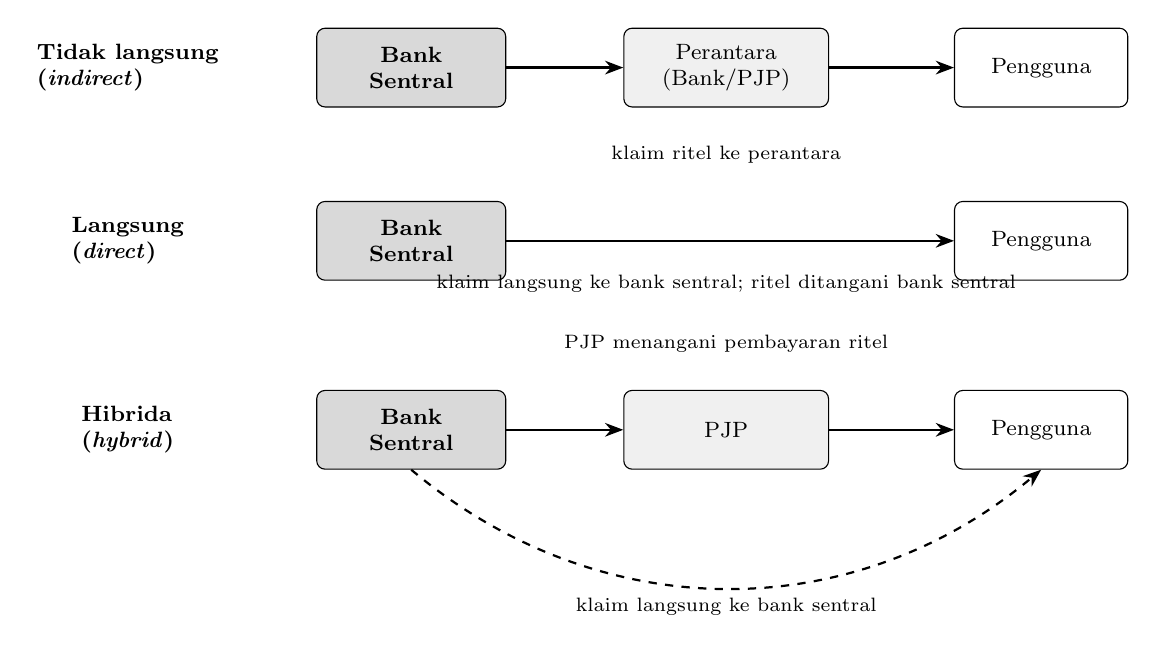
\begin{tikzpicture}[
  cb/.style={draw=black, fill=gray!30, rectangle, rounded corners=3pt,
    minimum width=2.4cm, minimum height=1.0cm, align=center, font=\footnotesize\bfseries},
  mid/.style={draw=black, fill=gray!12, rectangle, rounded corners=3pt,
    minimum width=2.6cm, minimum height=1.0cm, align=center, font=\footnotesize},
  usr/.style={draw=black, fill=white, rectangle, rounded corners=3pt,
    minimum width=2.2cm, minimum height=1.0cm, align=center, font=\footnotesize},
  lbl/.style={font=\footnotesize\bfseries, align=left},
  note/.style={font=\scriptsize, align=center},
  ar/.style={-{Stealth}, thick},
  ard/.style={-{Stealth}, thick, dashed},
]

%==== Baris 1: Tidak Langsung (Indirect / dua jenjang) ====
\node[lbl] at (-3.6, 2.2) {Tidak langsung\\(\textit{indirect})};
\node[cb]  (cb1)  at (0, 2.2) {Bank\\Sentral};
\node[mid] (int1) at (4.0, 2.2) {Perantara\\(Bank/PJP)};
\node[usr] (u1)   at (8.0, 2.2) {Pengguna};
\draw[ar] (cb1.east)  -- (int1.west);
\draw[ar] (int1.east) -- (u1.west);
\node[note] at (4.0, 1.1) {klaim ritel ke perantara};

%==== Baris 2: Langsung (Direct / satu jenjang) ====
\node[lbl] at (-3.6, 0.0) {Langsung\\(\textit{direct})};
\node[cb]  (cb2) at (0, 0.0) {Bank\\Sentral};
\node[usr] (u2)  at (8.0, 0.0) {Pengguna};
\draw[ar] (cb2.east) -- (u2.west);
\node[note] at (4.0, -0.55) {klaim langsung ke bank sentral; ritel ditangani bank sentral};

%==== Baris 3: Hibrida (Hybrid) ====
\node[lbl] at (-3.6, -2.4) {Hibrida\\(\textit{hybrid})};
\node[cb]  (cb3)  at (0, -2.4) {Bank\\Sentral};
\node[mid] (int3) at (4.0, -2.4) {PJP};
\node[usr] (u3)   at (8.0, -2.4) {Pengguna};
\draw[ar] (cb3.east)  -- (int3.west);
\draw[ar] (int3.east) -- (u3.west);
\draw[ard] (cb3.south) to[out=-40,in=-140] node[note,below]{klaim langsung ke bank sentral} (u3.south);
\node[note] at (4.0, -1.3) {PJP menangani pembayaran ritel};

\end{tikzpicture}%

\end{document}
